\documentclass[english]{article}
\usepackage[scaled]{helvet}
\renewcommand*\familydefault{\sfdefault}
\usepackage[T1]{fontenc}
\usepackage[utf8]{inputenc}
\usepackage[a4paper]{geometry}
\geometry{verbose,lmargin=2.5cm,rmargin=2.5cm}
\usepackage[table]{xcolor}
\usepackage{graphicx}
\graphicspath{{./}}

\usepackage{babel}
\usepackage{pdfpages}
%\usepackage{cite}
\usepackage[gen]{eurosym}
\usepackage{xcolor}
\usepackage{hyperref}
\usepackage[space]{grffile}
\begin{document}
\pagenumbering{gobble}
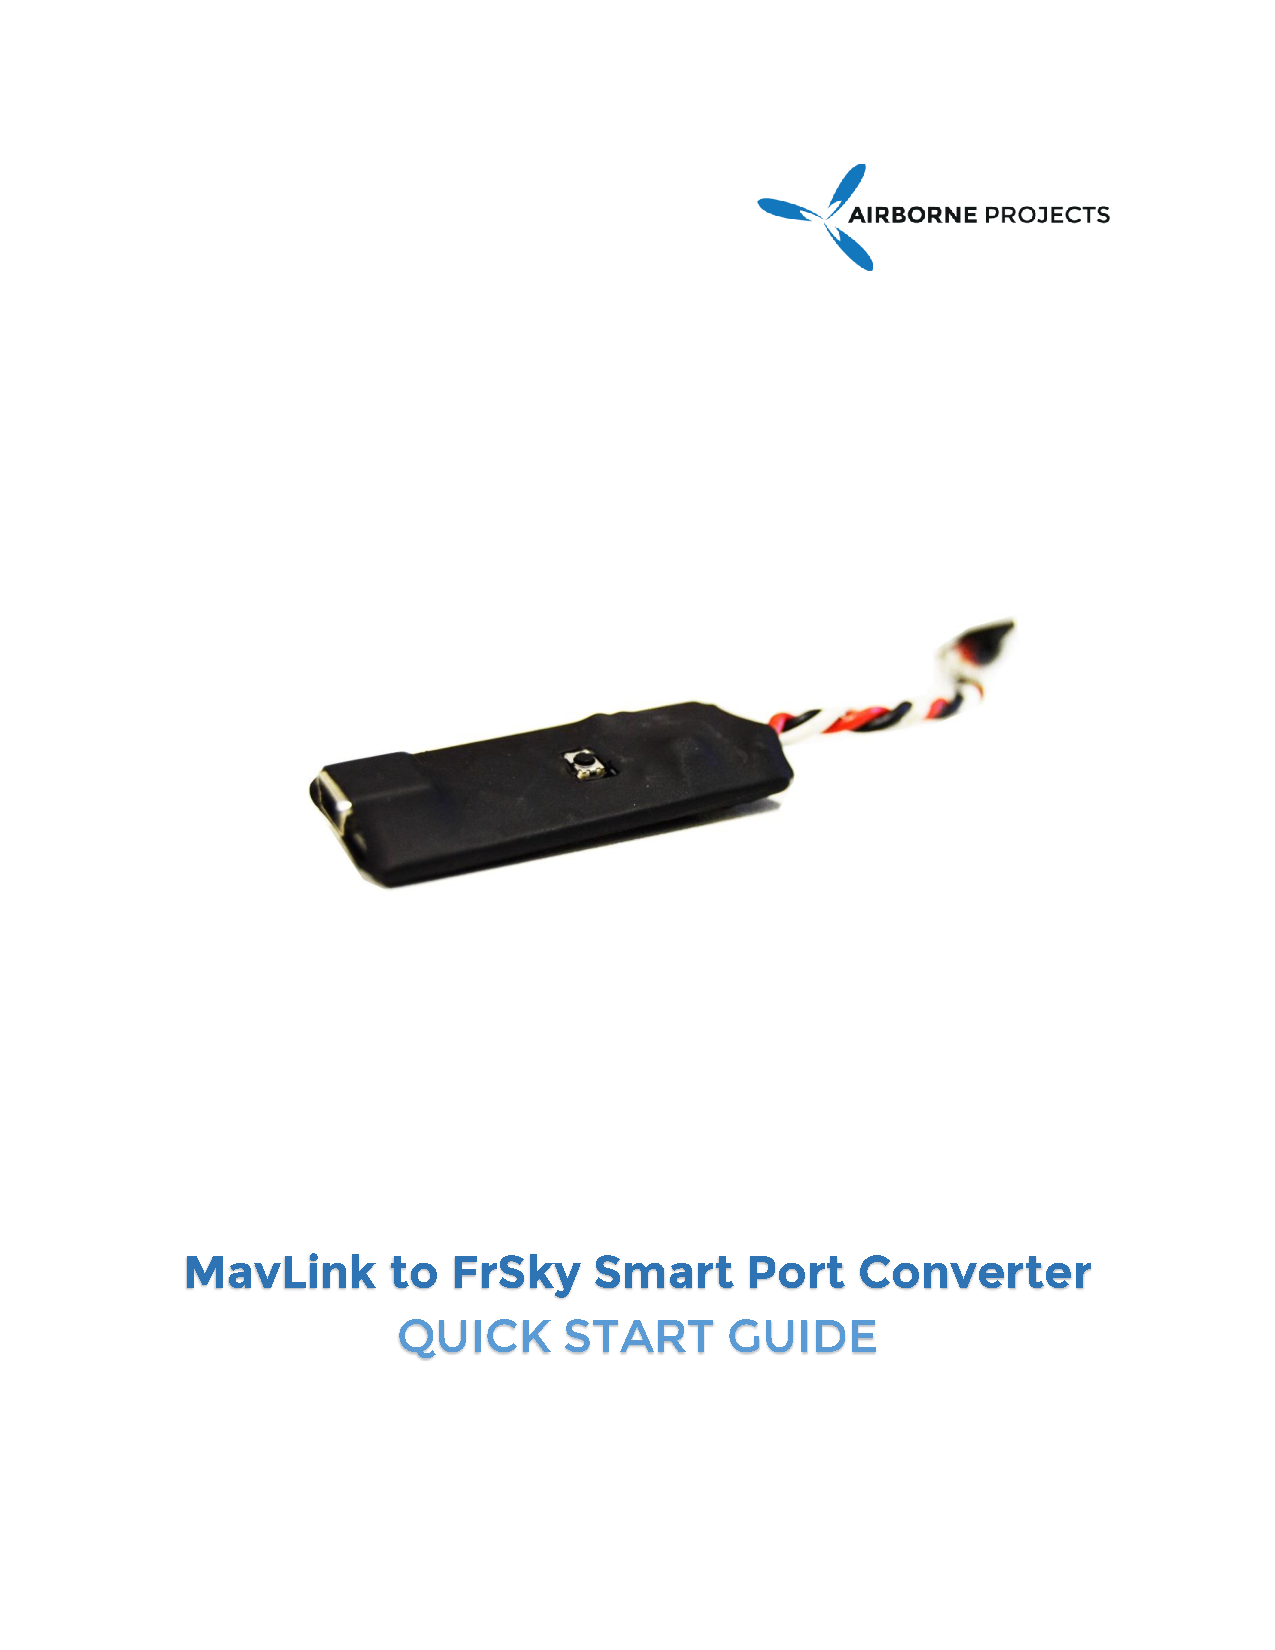
\includepdf{Cover}
\clearpage
\tableofcontents
\clearpage
\pagenumbering{arabic}
\setcounter{page}{1}
\section{Context}

This manual's goal is to get the Airborne Projects' "Mavlink to FrSky Smart Port Converter" working with OpenTX 2.1.X, where X is a version number higher or equal to 3. To accomplish this, converters sold before 21 of October of 2015 need to have their firmware upgraded.

The reason the Mavlink Converters firmware needs to be upgraded is due to the way OpenTX 2.1.X version changed the telemetry system. Even so, most of the important functionality remains operational with the pre-October 21st firmware, just with LUA scripts upgrades.

The firmware upgrade is not possible on the Mega's converter version because the USB-To-Serial chip needs to be disabled to work correctly with the APM Mega board. This is unfortunate and we provide a secondary workaround that involves flashing the Taranis with firmware compiled from the OpenTX repository master branch. This is because in versions up to 2.1.3 there was a bug in sensor naming. Airborne Projects provided a patch to OpenTX which was accepted and merged with the upcoming version of OpenTX.

\section{Getting Started}

This is a telemetry relay board that sits between the telemetry port of your APM or Pixhawk module and the Smart Port of your FrSky receiver sending your flight controller telemetry to your Taranis radio.

%\section{Parts}

%\begin{figure}[!h]
%	\centering
%	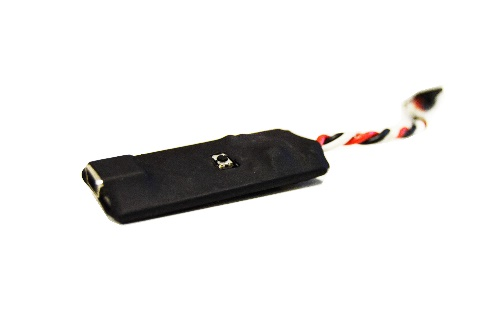
\includegraphics{Parts1.jpg}
%	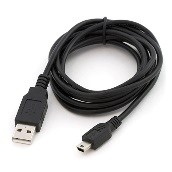
\includegraphics{Parts 2 Cable.jpg}
%\end{figure}

\section{Assumptions}

\begin{itemize}

\item The Taranis radio transmitter is bound to its receiver which is connected to the "MavLink
to FrSky SmartPort Converter” through its Smart Port;

\item A "MavLink to FrSky SmartPort Converter" module is connected to an APM telemetry
output, specifically the native APM / Pixhawk telemetry port;

\item The power to the "MavLink to FrSky SmartPort Converter" is supplied by the APM telemetry port;

\item The "MavLink to FrSky SmartPort Converter" has the firmware recommended by Airborne
Projects;

\item It is assumed you can connect to your APM module from the "Mission Planner" software
on Windows, even though the steps are similar for QGroundControl available in every PC
operating system;

\item It is assumed you have a Mini-USB cable.

\item You have the transmitter and receiver bound in D16 mode. This is very important as other modes do not work with telemetry. Check \url{https://www.youtube.com/watch?v=1IYg5mQdLVI} for details on how to do it.

\item You have downloaded the zip file containing the HEX file and the LUA scripts from \url{https://www.airborneprojects.com/wp-content/uploads/2015/08/frsky\_telemetry\_workaround.zip}

\item You have downloaded XLoader from \url{http://russemotto.com/xloader/XLoader.zip} so you can program the HEX file into the Mavlink Converter.

\end{itemize}

\section{How to Enable Telemetry on Mission Planner}

\begin{enumerate}

\item Select the "Config/Tuning" tab;
\item Select "Full Parameter Tree";
\item For the secondary telemetry port configurations find the command node SR1. For information about what this parameters go to ArduCopter’s SR1 official documentation;
\item In SR1.\footnote{SR1 or SERIAL1 is a placeholder for any of the telemetry channels and can be taken as SRa or SERIALa, where “a” is the number of the telemetry port where the converter is connected.
} node set:
\begin{enumerate}
\item SR1\_EXT\_STAT 10
\item SR1\_EXTRA1 0
\item SR1\_EXTRA2 10
\item SR1\_EXTRA3 3
\item SR1\_PARAMS 1
\item SR1\_POSITION 1
\item SR1\_RAW\_CTRL 0
\item SR1\_RAW\_SENS 10
\item SR1\_RC\_CHAN 0
\end{enumerate}


\item Find the command node SERIAL1 and set:
\begin{enumerate}
\item SERIAL1\_BAUD 57
\item SERIAL1\_PROTOCOL 1
\end{enumerate}
\item In the Writing part of the window find and click in "Write Params".

\end{enumerate}

\section{Loading the Lua telemetry files to the Taranis remote}

\begin{enumerate}

\begin{figure}[hb!]
\centering
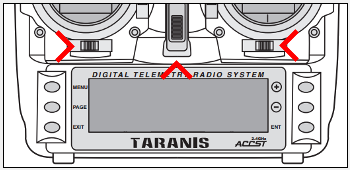
\includegraphics{Taranis Schematic.png}
\caption{Booloader mode}
\end{figure}

\item Ensure you have your Taranis transmitter turned off;

\item Enter bootloader mode by sliding both horizontal trims, each under the main sticks, to the center of the remote and then turn on the radio;

\item A Taranis bootloader screen should show. If you still hear the normal greeting message you have not entered the Bootloader Screen, thus you should repeat the previous steps in this section;

\item Without selecting any menu connect the USB mini to the back of your Taranis and the USB to your computer. The text "USB Connected" will be displayed. If you turn on the USB with the Radio off it will not be able to turn on until you disconnect it;

\item In your computer there should be a notification that 2 Removable Drives have been added
to your computer. One says "Taranis" and the other has a non-descriptive. You should
choose the one with the non-descriptive name. One way to spot it is that the one with
.BIN files is the wrong drive;

\item  In the root of the correct drive there should be several folders but you should find one
called "Scripts". Don't exit this directory because you will past files to it.

\item Inside the "SCRIPTS" directory you should have another called "TELEMETRY" If you don't, create it and go inside it;

\item  Unpack the downloaded .zip file mentioned in the Assumptions section to your desired location. This file contains the firmware source code, the converter HEX file as well as the Lua telemetry scripts;

\item In the directory where you unpacked it, walk the directory tree "Lua/2\_1\_x" and copy both telem1.lua and telem2.lua to the "TELEMETRY" folder mentioned before.

\item Safely remove both drives and turn on your Radio and remove the USB cable.

\item Turn on your radio normally.

\item From the initial screen screen press "MENU" and then long press "PAGE" button to go to the "TELEMETRY" page.

\item Scroll down the "TELEMETRY" page until you find the option "Discover new sensors". Toggling this option allows the radio to enable or disable new sensor discovery. For Airborne Projects' Mavlink Converter 17 sensors should be discovered, with no name repetitions.

\item  Stop the discovery when 17 sensors are discovered.

\item Scroll further down until you find the text "Screen 1". On "Screen 1" press "ENT" and with the "+" or "-" keys navigate the menu until you find the text "Script". When you find it press "ENT".

\item In the same row, in the next column press "ENT". A menu with the script names you have placed in the "TELEMETRY" folder will appear. For the "Screen 1" you should select "telem1"

\item Repeat the same step on "Screen 2" but now select telem2.

\item Press "EXIT" until you are in the initial screen again.

\item Long pressing "PAGE" will take you to the telemetry screen with the most information. Pressing again will take you to the 2nd telemetry screen which contains the GPS coordinates and a log of the text messages issued by the Ardupilot.

\end{enumerate}

\subsection{Troubleshooting}

Sometimes for a yet unknown reason the sensors are considered "bad" by the 2.1.X firmware and they need to be "Discovered" again. This may happen when the Ardupilot is disarmed or when the converter is turned off manually and then reconnected.

To solve the situation above just follow the steps to "Discover" new sensors but deleting the inactive ones before. One way to know to be sure there are no "dangling" inactive sensors is that no more than 17 sensors should be displayed. 

No further manual sensor configuration should be necessary as the LUA scripts were designed to workaround the default values that OpenTX presents.

If you have a configuration problem that you cannot solve please let us know and contact us.

\section{Loading new firmware into the Converter}

This section only applies if the converter's firmware is from a previous date than 21 of October and a Pixhawk or Navio version.

\begin{enumerate}
\item Disconnect the converter from any device including from the SmartPort plug and from the DF13 telemetry plug. \textbf{This is very important.}

\item Connect the Mini USB plug to the Converter's USB port and wait for it to be recognized by Windows. It should be recognized as an Arduino.

\item Launch XLoader and configure it according to Figure \ref{fig:xloader}, taking into account the path where you extracted the zip file and thus where the HEX file is. The .HEX file is the new firmware to be loaded into the converter.

\item Hit upload.

\begin{figure}[h!]
\centering
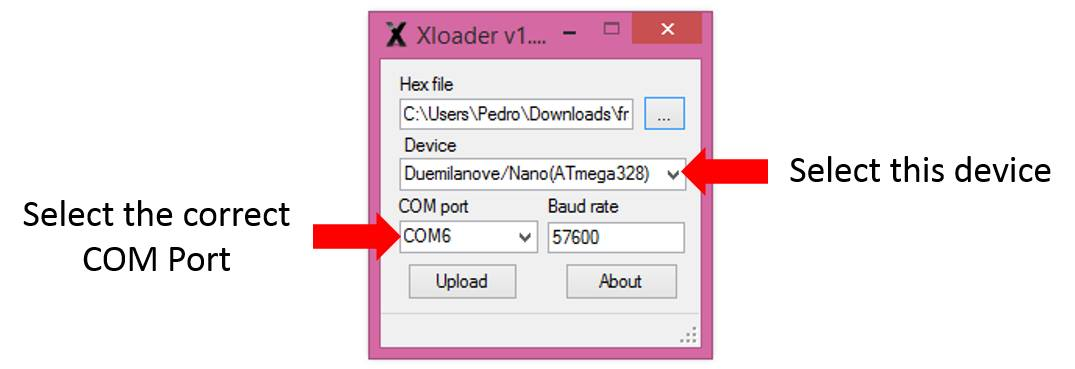
\includegraphics[width=1.0\textwidth]{XLoader}
\caption{XLoader configuration}
\label{fig:xloader}
\end{figure}

\end{enumerate}

A good way to check if the update was successful is to see if the LED light blinks periodically. If it does a valid firmware is inside. If not, no hard trouble can happen and just trying to correctly follow the above steps will get your situation solved. It is now time to connect the Converter back to your Taranis SmartPort and Telemetry Port.

\section{GUI Description}

\begin{figure}[h!]
	\centering
	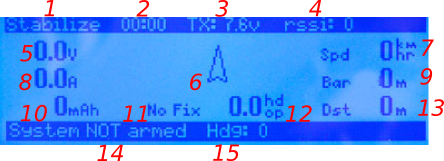
\includegraphics{LCD Description}
	\caption{LCD description}
\end{figure}

\begin{enumerate}

\item APM current Flight Mode
\item Taranis Timer
\item Taranis Battery Voltage
\item RSSI / radio signal quality
\item Airframe battery voltage (should be calibrated through Mission Planner for this to be meaningful)
\item Relative Heading Arrow. When system is not armed points measured heading. When armed, displays the heading relative to the arming orientation
\item GPS speed. Only shows when GPS is acquired or enabled
\item Measured battery current draw (similar to voltage meter must be calibrated);
\item Barometric Altitude (altitude measured by barometric sensor)
\item Integrated power over time (be sure you have both voltage and current calibrated before relying on this)
\item GPS status or number of satellites available
\item HDOP (horizontal dilution of precision). A measure of the geometric quality of a GPS satellite configuration in the sky. The lower the better
\item Distance from first GPS position received by the Taranis
\item Arming status emitted by APM
\item Numeric representation of the arrow angle

\end{enumerate}

\section{Converter Description}

\begin{figure}[h!]
        \centering
        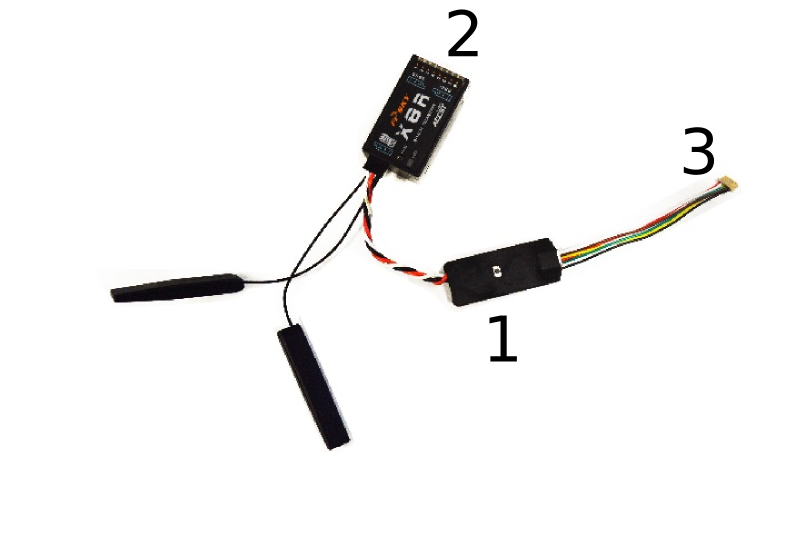
\includegraphics[width=0.7\textwidth]{Assembled Converter}
	\caption{Assembled Converter}
\end{figure}

\begin{enumerate}

\item MavLink to FrSky SmartPort Converter
\item FrSky receiver with Smart Port (telemetry compatible)
\item UART/Telemetry cable (only on UART version)

\end{enumerate}

\section{Specifications}

\begin{itemize}

\item Translation of Mavlink messages to FrSky Smart Port format
\item User friendly telemetry LUA script that detects APM arming to provide relative heading regarding arming orientation, direct from the APM IMU
\item Cheaper alternative to Teensy
\item Lower Power Consumption (20mA)
\item Input voltage range: 5V-10V (powered by receiver SMART Port)
\item Heat-shrinked wrapping to afford debris protection without compromising weight

\end{itemize}

\section{Further Information}

For more information about the loaded firmware source files and scripts, visit \url{https://github.com/ptsneves/FrSkyTelemetry}.

For customer support, contact us at \url{info@airborneprojects.com}.

\section{APM Mega pre 21st of October workaround for OpenTX 2.1.X}

\subsection{Problem}

The original Airborne Projects Converter Firmware is not compatible with OpenTX 2.1.3 because one of sensor, namely "Battery remaining" is assigned the same identifier name as the Satellites visible sensor. This happens because in OpenTX 2.1.3 Frsky Sensor "Temp1" and "Temp2" are given the same "temp" identifier, causing an ambiguity. This breaks the way 2.0.X sensors were named, but most importantly breaks consistency with similar conventions like "A0", "A1", etc. To solve this problem Airborne Projects produced a patch that is already merged with the "master" branch of OpenTX and is due to be part of the next minor 2.1.X OpenTX version. This situation is out of Airborne Projects control and we cannot do anything about it. You can confirm the merging in OpenTX official repository at \url{https://github.com/opentx/opentx/pull/2955}

The converters firmware cannot be upgraded because the way the APM Mega Serial multiplexer interacts with the CH340 USB-to-Serial requiring us to cut it's traces and remove some resistors, effectively making it non-reprogramable without hardware modifications. As the scripts have no way of knowing which sensor is which only an upgrade to the Taranis Plus firmware can solve this problem.

\subsection{Patched OpenTX Firmware}

This is done at your own risk. Please contact Airborne Projects for a patched Taranis firmware that corrects the ambiguity.

\end{document}
